\section{Les arbres de décisions}
\label{chap4.section2}
Un arbre de décision est une représentation d'un processus de prise de décision séquentiel qui prend un vecteur de paires \textbf{attribut-valeur} et renvoie une sortie unique, une « décision ». Un arbre de décision est un modèle non paramétrique qui prend sa décision en effectuant une séquence de tests sur les valeurs des attributs d'un exemple donné, en commençant par la racine et en suivant la branche appropriée jusqu'à atteindre une feuille (fin d'un chemin). Chaque nœud interne de l'arborescence correspond à un test de la valeur de l'un des attributs d'entrée, les branches du nœud sont étiquetées avec les valeurs possibles de l'attribut, et les feuilles précisent quelle valeur doit être renvoyée par la fonction à la fin d'un chemin donné.

Les valeurs d'entrée peuvent être discrètes ou continues, même si les arbres de décision sont généralement utilisés avec des attributs/prédicateurs catégoriques, nous pouvons tirer parti du seuillage ou de tout autre type d'encodage pour utiliser des attributs à valeur continue comme entrée. Par exemple, âge entre 0 et 40 => catégorie-1, âge > 40 => catégorie-2). Cependant, les résultats ou les décisions doivent provenir d’un ensemble fixe de valeurs, appélées des \textbf{classes}. Lorsque les classes sont simplement vrai/faux ou rembousera/remboursera-pas (le prêt), nous appelons cela: classification booléenne ou binaire.

Un arbre de décision peut techniquement renvoyer des valeurs continue, on les appelle \textbf{arbres de régression}, ils fonctionnent de la même manière que les arbres de décision, dans le sens où ils suivent un chemin en fonction des valeurs des attributs mais au lieu de continuer ce processus jusqu'à ce qu'ils atteignent une « feuille », ils renvoient une prédiction qui est la moyenne des étiquettes dans le dernier nœud. Par exemple, si les autres points de données qui ont les mêmes valeurs d'attribut que celui pour lequel nous voulons prédire une étiquette ont les étiquettes suivantes: \(7, 7, 10, 9\). L'arbre de régression renverra alors \(\frac{7 + 7 + 10 + 9}{4} = 8.25\). Dans certains cas il n'y a tout simplement plus d'attributs pour différencier les exemples, dans ce genre de cas un arbre de décision peut agir comme un arbre de régression ou juste retourner l'étiquette la plus fréquente dans le dernier nœud, avec l'exemple précédent un arbre de décision retournerait \(7\).

Un arbre de décision est donc équivalent à l'expression logique suivante: \[Sortie =(chemin_1 \lor chemin_2 \lor chemin_3 ...)\] où chaque \(chemin_i\) est une conjonction de la forme (\(A_m = v_x \land A_n = v_y \land ...\)) de tests de valeur d'attribut correspondant à un chemin de la racine à une feuille. Ainsi, toute fonction en logique propositionnelle peut être exprimée sous forme d’arbre de décision.

Ok, un arbre de décision prend une décision en suivant un chemin décidé par des tests sur les valeurs des attributs d'un exemple, mais comment construire ces chemins? En fait, le problème n’est pas de savoir comment construire un arbre de décision mais comment « l’apprendre » à partir des données. En effet, le problème est que si nous voulons simplement un arbre de décision, il n’existe pas qu’une seule façon de le construire et il n’y a pas qu’un seul arbre qui corresponde à un ensemble de données donné. Par exemple, si nous devions programmer un arbre de décision, nous pourrions utiliser n'importe quel attribut de notre ensemble de données comme racine et diviser les données selon n'importe quel aspect ou critère qui nous intéresse. Cela pourrait donner lieu à des centaines d’arbres possibles pour un ensemble de données, mais tous ne sont pas de « bons arbres de décision ».

\subsection{Construire un arbre de décision par intuition}
\label{chap4.sec2.sub1}
Pour l'illustration, considérons l'ensemble de données présenté dans le tableau \ref{tab:tab1}. Cet ensemble est constitué de cinq attributs ou prédicateurs, le but étant de prédire le risque d'un patient atteint du covid-19 avec trois classes: SOFT\_COVID (le patient devrait aller bien et a besoin de moins d'attention), STRONG\_COVID (le patient est en danger et a besoin de plus d'attention) et DEAD (le patient doit être considéré comme une urgence et pourrait mourir). Ce petit ensemble de données n'est là que pour illustrer le fonctionnement des arbres de decisions et expliquer les concepts, je l'ai choisi pour cet exemple parce que toutes les variables sont catégoriques ce qui va simplifier la représentation de l'arbre, il a été générer par un réseau de neuronnes artificiel que j'ai entraîner sur d'autres données du monde réel (\cite{diarra2023covid}). Pour simplifier on considerera juste dix exemples d'entraînements et cinq attributs, cela permettra de pouvoir faire les calculs à la main.

\begin{table}
    \centering
    \begin{tabular}{ |c|c|c|c|c|c|c| }
        \hline
        ID & SEX & PNE & PRE & AGE & DIA & LAB \\
        \hline
        0 & 2 & 1 & 2 & 73 & 1 & 2 \\
        \hline
        1 & 1 & 2 & 2 & 39 & 2 & 0 \\
        \hline
        2 & 2 & 1 & 2 & 46 & 2 & 1 \\
        \hline
        3 & 1 & 1 & 2 & 74 & 2 & 2 \\
        \hline
        4 & 2 & 1 & 2 & 1 & 2 & 1 \\
        \hline
        5 & 1 & 2 & 2 & 46 & 2 & 0 \\
        \hline
        6 & 1 & 2 & 2 & 24 & 2 & 0 \\
        \hline
        7 & 2 & 2 & 2 & 54 & 1 & 2 \\
        \hline
        8 & 1 & 1 & 1 & 37 & 2 & 1 \\
        \hline
        9 & 1 & 2 & 1 & 42 & 2 & 0 \\
        \hline
    \end{tabular}
    \caption{Données synthétiques (Covid Classification)}
    \label{tab:tab1}
\end{table}

\textbf{Signification des prédicateurs}:

\begin{itemize}
    \item SEX: 1=femme, 2=homme
    \item PNEUMONIE (PNE): si le patient présente déjà une inflammation pulmonaire ou non
    \item ENCEINTE (PRE): si la patiente est enceinte ou non
    \item ÂGE: l'âge du patient
    \item DIABÈTE (DIA): si le patient est diabétique ou non
    \item PRÉDICTION (LAB): 0 (SOFT\_COVID), 1 (STRONG\_COVID), 2 (DEAD).
\end{itemize}

Un arbre de décision pour ce problème de classification est la représentation de n'importe quelle fonction logique capable de distinguer ces exemples. N'importe quel attribut de ce tableau peut être la racine d'un arbre (une solution), nous pouvons donc facilement construire un arbre qui classifie correctement ces exemples. Un arbre de décision possible pour ce problème de classification de covid est montré dans la figure \ref{fig:fig3}. 

\begin{figure}
    \centering
    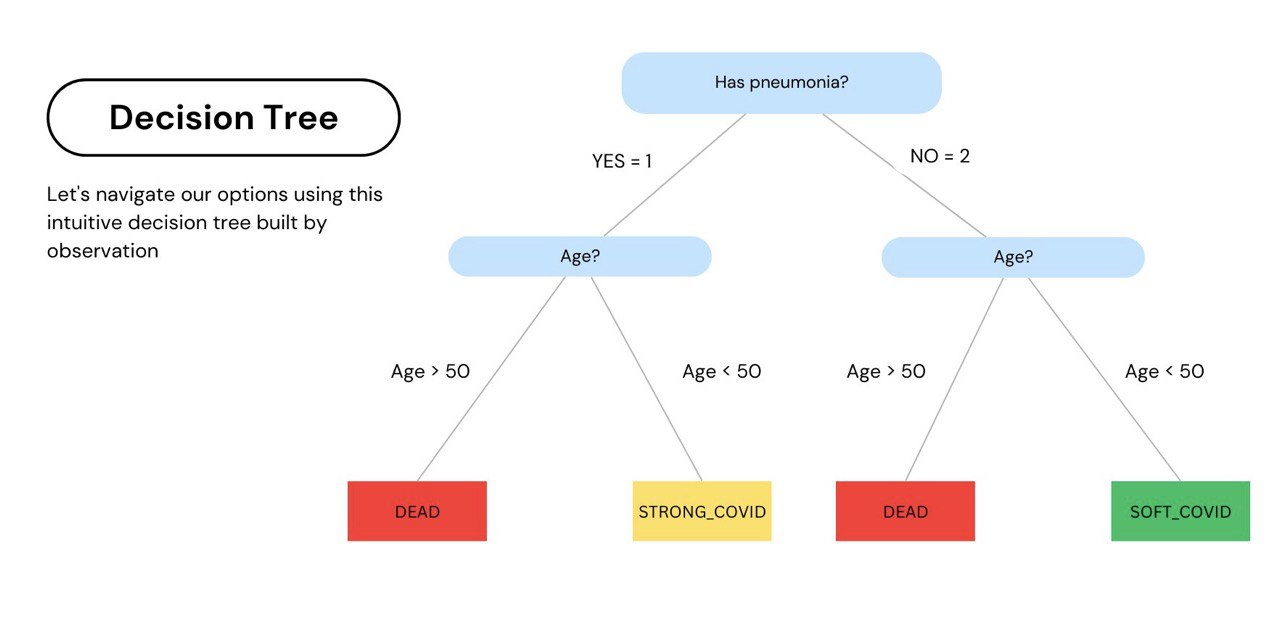
\includegraphics[width=0.75\linewidth]{images/DecisionTree1.jpg}
    \caption{Un arbre de décision construit en choisissant l'attribut qui divise l'ensemble de données en deux sous-ensemble de taille égale comme racine}
    \label{fig:fig3}
\end{figure}

Avec l'arbre montré dans la figure \ref{fig:fig3}, on s'est arrêté parce qu'il ne restait plus aucun exemple d'entraînement qui ne soit pas classifiable avec cet arbre mais en pratique on peut toujours ajouter des nœuds. Simplement construire un arbre de décision n'est donc pas compliqué. Le problème est que nous avons construit cet arbre dans le but de classifier juste ces dix exemples d'entraînements or notre but est d'obtenir un modèle qui est appris à généraliser des connaissances tirées du jeu de données pour pouvoir prédire les étiquettes d'autres exemples, c'est cela la tâche de l'apprentissage supervisé, il s'agit de se rapprocher au maximum de la fonction inconnue qui a générée les données (dans ce cas précis un réseau de neuronnes artificiel) pas de mémoriser l'ensemble d'entraînement.

\subsection{Apprendre un arbre de décision}
\label{chap4.sec2.sub2}
L’essence de l’apprentissage dans les arbres de décision réside dans la création d’un modèle capable de prédire avec précision les étiquettes de nouvelles données invisibles tout en restant simple et relativement petit (\cite{RussellNorvig2020}). Apprendre un arbre de décision consiste à trouver l'attribut le plus important pour diviser les données à chaque étape, de la racine au dernier nœud. Par « attribut le plus important », nous entendons celui qui fait le plus de différence dans la classification d’un exemple. En termes simples, l'attribut le plus important d'un ensemble de données est celui qui divise l'ensemble de données en groupes aussi homogènes que possible de part ses valeurs. Traditionnellement on utilise le concept de gain d'information expliqué dans la section \ref{chap3.sec1.sub1} pour déterminer l'attribut le important à chaque nœud, même si toute autre fonction pourrait être utiliser. L'attribut le plus important est donc une autre appelation de l'attribut le plus informatifs.

\subsection{Algorithme}
\label{chap4.sec2.sub3}
Une fois que l'on a trouvé l'attribut le plus informatif, on divise l'ensemble de données en sous-ensembles en fonction des valeurs de cet attribut. C'est une mannière de diviser recursivement le problème de base en plus petits sous problèmes pour lesquels on peut appliquer l'algorithme suivant:

\begin{enumerate}
    \item Si les exemples restants sont tous dans la même catégorie (de la même classe), alors nous avons terminé: nous pouvons renvoyer cette classe comme décision.
    \item Sinon Si les exemples restants sont hétérogènes (de classes différentes), choisir le meilleur attribut pour créer un nouveau nœud.
    \item S'il ne reste plus d'exemples, cela signifie qu'aucun exemple n'a été observé pour cette combinaison de valeurs d'attribut, et nous renvoyons la valeur de sortie la plus courante de l'ensemble d'exemples utilisés lors de la construction du parent du nœud (nous pouvons également implémenter n'importe quel autre logique dans ce cas).
    \item S'il ne reste plus d'attributs, mais des exemples de classes différentes, cela signifie que ces exemples ont exactement la même description, mais des classifications différentes. Cela peut se produire en raison d'une erreur; parce que l'environnement est non déterministe; ou parce que nous n’avons pas ou ne pouvons pas observer un attribut qui distinguerait les exemples. Le mieux que nous puissions faire est de renvoyer la valeur de sortie la plus courante des exemples restants.
\end{enumerate}

En appliquant l'algorithme ci dessus aux données de la table \ref{tab:tab1} on obtient l'arbre illustré dans la figure \ref{fig:fig4}. La principale différence entre cet arbre et l'arbre de la figure \ref{fig:fig3} est que celui là est construit en fonction du gain d'information et est donc capable de changer pour s'adapter à d'autres ensemble de données ou simplement un plus grand ensemble. On peut donc dire que cet algorithme peut « apprendre » des données. Pour la tâche de prédiction des défauts de paiement je n'ai pas directement implémenté d'arbres de décisions mais d'autres algorithmes basés sur les arbres de décisions, donc une compréhension des arbres de décisions (offerte dans cette section) me permettra d'être plus concis dans l'explication des algorithmes de la Forêt aléatoire et du boost de gradient.

\begin{figure}
    \centering
    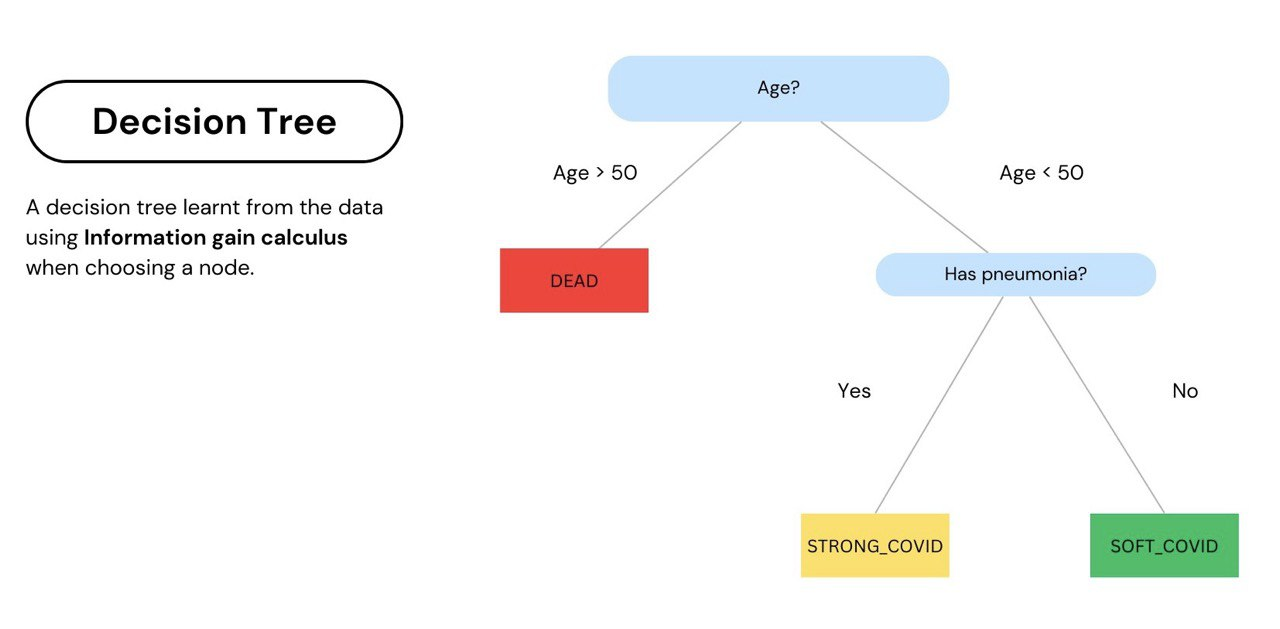
\includegraphics[width=0.75\linewidth]{images/DecisionTree2.jpg}
    \caption{Un arbre de décision construit grâce au gain d'information}
    \label{fig:fig4}
\end{figure}